\subsection*{Hypothesis 6}

- The larger the number of books published for a category, the higher the review score.\\ 
- The larger the number of books published by publishers, the higher the review score.\\

\noindent
\textbf{Description and Results}
All the data cleaning and transformation steps were performed using MongoDB with the aggregation pipeline, to have a more efficient and faster computation.\\
Specifically the data cleaning steps were performed using the \textit{\$match} operator, while the data transformation steps were performed using the \textit{\$group} operator with \textit{\$avg} operation.
Finally a \textit{\$project} operator was used to select the fields of interest. To reduce bias, we removed the categories having less than 50 books and the publishers having less than 20 books.\\
The results are shown in Table \ref{tab:h6_correlations}.\\
\textbf{Conclusion:} The hypotheses are falsified since the metrics shows no correlation between the two variables in both cases.

\begin{table}[H]
    \centering
    \caption{Correlation Values and P-values for Categories and Publishers}
    \begin{tabular}{|c|c|c|}
    \hline
    \textbf{Variable} & \textbf{Correlation Value} & \textbf{P-value} \\
    \hline
    Category & -0.0806 & 0.558 \\
    \hline
    Publisher & -0.0673 & 0.151 \\
    \hline
    \end{tabular}
    \label{tab:h6_correlations}
\end{table}

\vspace{0.5cm}
\noindent 
\textbf{Curiosity}
We performed two complex MongoDB queries (reported as example in section 'Code') to answer to two questions:\\
\begin{itemize}
    \item Which are the best publishers? (i.e. capable of getting avg scores above 4.5 in lots of categories)
    \item In which categories are the best publishers focused?
\end{itemize}

The results are reported in Figure \ref{fig:h6_which_best} and Figure \ref{fig:h6_where_best}.

\begin{figure}[H]
    \centering
    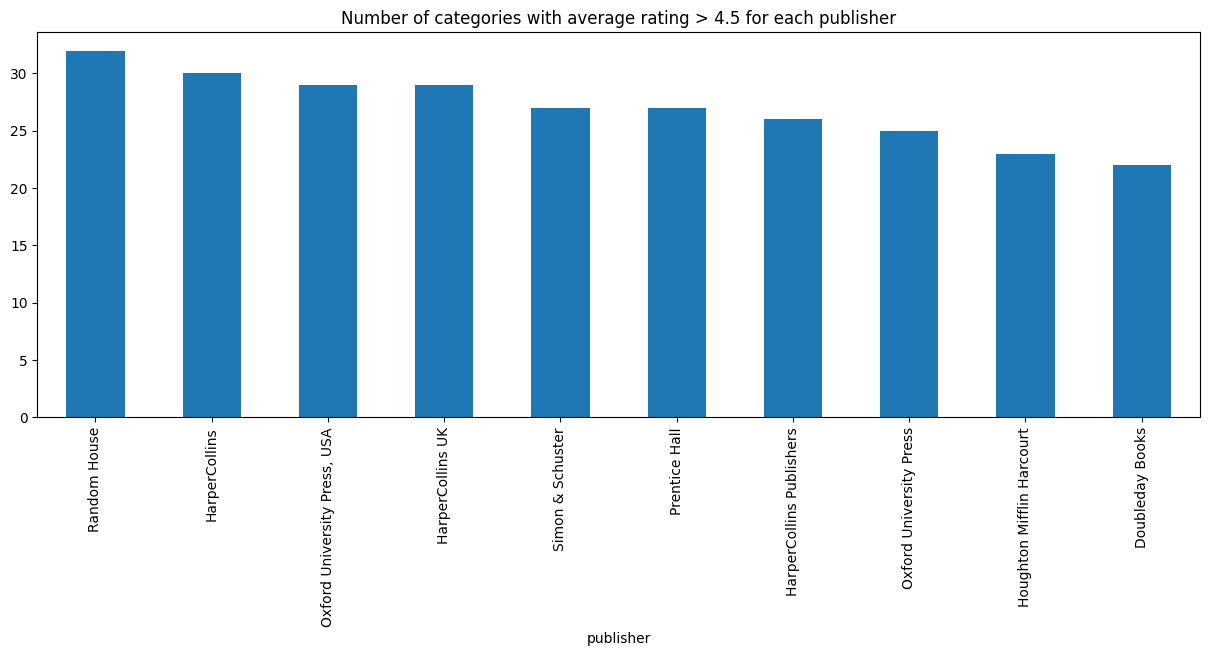
\includegraphics[width=0.5\textwidth]{./figures/h6_which_best.png}
    \caption{Which are the best publishers?}
    \label{fig:h6_which_best}
\end{figure}

\begin{figure}[H]
    \centering
    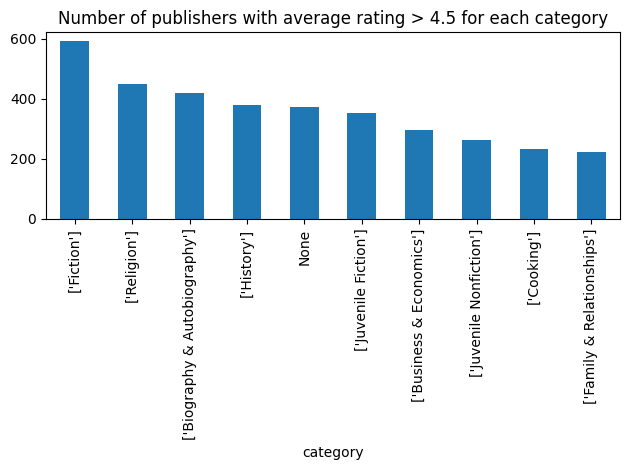
\includegraphics[width=0.5\textwidth]{./figures/h6_where_best.png}
    \caption{In which categories are the best publishers focused?}
    \label{fig:h6_where_best}
\end{figure}